% ============================================================
% Module 05: RAG Fundamentals — REWORKED (concept + visualization, code-free)
% Custom Navasena Dark Beamer Theme
% Compiler: xelatex
% ============================================================
\documentclass[aspectratio=169,t]{beamer}

% ---- Fonts (xelatex) ----------------------------------------
\usepackage{fontspec}
\usepackage[sfdefault]{FiraSans}

% ---- Core packages ------------------------------------------
\usepackage{graphicx}
\usepackage{tikz}
\usetikzlibrary{positioning, shapes.geometric, arrows.meta, calc}
\usepackage{pgfplots}
\pgfplotsset{compat=1.18}
\usepackage{amsmath}
\usepackage{booktabs}
\usepackage{colortbl}
\usepackage{xcolor}

% ============================================================
% COLOR PALETTE (Navasena dark theme)
% ============================================================
\definecolor{nvbg}{HTML}{1A1A2E}
\definecolor{nvdark}{HTML}{1A1A2E}
\definecolor{nvcard}{HTML}{2D2D44}
\definecolor{nvgreen}{HTML}{76B900}
\definecolor{nvlightgreen}{HTML}{A3D944}
\definecolor{nvwhite}{HTML}{FFFFFF}
\definecolor{nvgray}{HTML}{AAAACC}
\definecolor{nvdarkcard}{HTML}{23233A}
\definecolor{nvred}{HTML}{EF5350}
\definecolor{nvorange}{HTML}{FF6F00}
\definecolor{nvblue}{HTML}{42A5F5}

% ============================================================
% BEAMER THEME — NAVASENA DARK
% ============================================================
\usetheme{default}
\usecolortheme{default}

\setbeamercolor{background canvas}{bg=nvbg}
\setbeamercolor{normal text}{fg=nvwhite}
\setbeamercolor{frametitle}{fg=nvwhite, bg=nvbg}
\setbeamercolor{framesubtitle}{fg=nvgray, bg=nvbg}
\setbeamercolor{title}{fg=nvgreen}
\setbeamercolor{author}{fg=nvgray}
\setbeamercolor{date}{fg=nvgray}
\setbeamercolor{item}{fg=nvgreen}
\setbeamercolor{subitem}{fg=nvlightgreen}
\setbeamercolor{subsubitem}{fg=nvgray}
\setbeamercolor{block title}{fg=nvwhite, bg=nvcard}
\setbeamercolor{block body}{fg=nvwhite, bg=nvcard}

\setbeamertemplate{footline}{%
  \hbox{%
    \begin{beamercolorbox}[wd=\paperwidth,ht=2.5ex,dp=1ex,leftskip=2em]{author in head/foot}%
      \color{nvgray}\small\textbf{RAG Fundamentals} \hfill \insertframenumber\,/\,\inserttotalframenumber
    \end{beamercolorbox}%
  }%
}
\setbeamertemplate{navigation symbols}{}

% ============================================================
% CUSTOM COMMANDS
% ============================================================
% \acttitle{N}{Title}{Subtitle}
\newcommand{\acttitle}[3]{%
  \begin{frame}[plain]
    \vspace{1.5cm}
    \begin{center}
      {\color{nvgreen}\Huge\bfseries Act #1}\\[1.2em]
      {\color{nvwhite}\Huge #2}\\[0.8em]
      {\color{nvgray}\Large #3}
    \end{center}
  \end{frame}%
}
% \takeaway{...}  — green one-line summary box
\newcommand{\takeaway}[1]{%
  \vspace{0.3em}
  \begin{beamercolorbox}[rounded=true,shadow=false,sep=6pt]{block body}
    \centering\small\color{nvlightgreen}#1
  \end{beamercolorbox}%
}

\title{RAG Fundamentals}
\subtitle{Navasena Gen-ML Course}
\author{Navasena AI}
\date{}

% ============================================================
\begin{document}

% ── Slide 1 — Title ───────────────────────────────────────
\begin{frame}[plain]
  \vspace{1.0cm}
  \begin{center}
    {\color{nvgreen}\Huge\bfseries Module 05}\\[0.9em]
    {\color{nvwhite}\Huge\bfseries RAG Fundamentals}\\[0.5em]
    {\color{nvgray}\Large Ground $\to$ Ingest $\to$ Retrieve $\to$ Ukur $\to$ Skala $\to$ Ngobrol $\to$ Sitasi $\to$ Deploy}\\[1.6em]

    
\begin{tikzpicture}[scale=0.85, every node/.style={transform shape},
        b/.style={draw=nvgreen, fill=nvcard, rounded corners=6pt, text=white, font=\small, minimum width=2.0cm, minimum height=0.9cm, align=center}]
      \node[b] (q) {Pertanyaan};
      \node[b, right=0.7cm of q] (r) {Retrieve};
      \node[b, right=0.7cm of r] (k) {Konteks};
      \node[b, right=0.7cm of k] (g) {Generate};
      \node[b, right=0.7cm of g, draw=nvorange] (a) {Jawaban};
      \draw[->,thick,color=nvgreen] (q)--(r);
      \draw[->,thick,color=nvgreen] (r)--(k);
      \draw[->,thick,color=nvgreen] (k)--(g);
      \draw[->,thick,color=nvorange] (g)--(a);
    \end{tikzpicture}

    \vspace{0.8em}
    {\color{nvgray}\small 8 notebook $\cdot$ gratis di Colab Tesla T4 16GB $\cdot$ Navasena AI $\cdot$ 2026}
  \end{center}
\end{frame}

% ── Slide 2 — Peta perjalanan ─────────────────────────────
\begin{frame}{Peta Perjalanan}
  \framesubtitle{Dari satu jawaban sederhana sampai layanan RAG siap-deploy}
  \begin{center}
  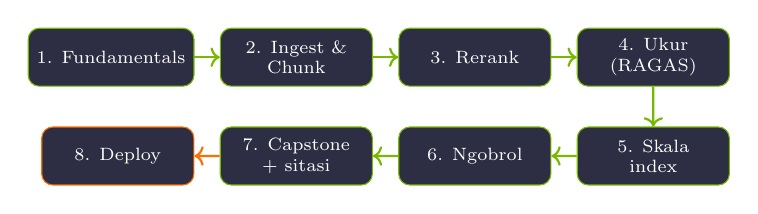
\begin{tikzpicture}[scale=0.92, every node/.style={transform shape},
      s/.style={draw=nvgreen, fill=nvcard, rounded corners=4pt, text=white, font=\scriptsize, minimum width=2.1cm, minimum height=0.8cm, align=center}]
    \node[s] (a) {1. Fundamentals};
    \node[s, right=0.35cm of a] (b) {2. Ingest \&\\Chunk};
    \node[s, right=0.35cm of b] (c) {3. Rerank};
    \node[s, right=0.35cm of c] (d) {4. Ukur\\(RAGAS)};
    \node[s, below=0.55cm of d] (e) {5. Skala\\index};
    \node[s, left=0.35cm of e] (f) {6. Ngobrol};
    \node[s, left=0.35cm of f] (g) {7. Capstone\\+ sitasi};
    \node[s, left=0.35cm of g, draw=nvorange] (h) {8. Deploy};
    \draw[->,thick,color=nvgreen] (a)--(b); \draw[->,thick,color=nvgreen] (b)--(c); \draw[->,thick,color=nvgreen] (c)--(d);
    \draw[->,thick,color=nvgreen] (d)--(e); \draw[->,thick,color=nvgreen] (e)--(f); \draw[->,thick,color=nvgreen] (f)--(g);
    \draw[->,thick,color=nvorange] (g)--(h);
  \end{tikzpicture}
  \end{center}
  \takeaway{Slide ini tidak per-notebook --- kita susun per \textbf{konsep}. Tiap konsep adalah satu balok di peta ini.}
\end{frame}

% ════════════════════════════════════════════════════════
\acttitle{1}{Kenapa RAG?}{LLM pintar berbahasa, tapi bukan sumber kebenaran fakta}

% ── Masalah LLM ───────────────────────────────────────────
\begin{frame}{Dua Masalah LLM Polos}
  \framesubtitle{Kenapa LLM saja tidak cukup untuk menjawab fakta}
  \begin{columns}[T]
    \begin{column}{0.56\textwidth}
      \begin{itemize}
        \footnotesize
        \item LLM menjawab dari \textbf{ingatan} hasil pelatihannya saja
        \item[\textcolor{nvred}{$\bullet$}] \textbf{Halusinasi} --- mengarang jawaban yang meyakinkan tapi salah
        \item[\textcolor{nvred}{$\bullet$}] \textbf{Knowledge cutoff} --- tak tahu kejadian setelah waktu training
        \item Tak bisa membaca dokumen \textbf{internal} kantor/sekolahmu
        \item Untuk fakta terbaru / spesifik $\to$ jawaban tak bisa dipercaya
      \end{itemize}
    \end{column}
    \begin{column}{0.42\textwidth}
      \begin{center}
      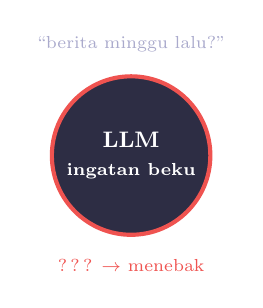
\begin{tikzpicture}[scale=0.9, every node/.style={transform shape}]
        \node[circle, draw=nvred, fill=nvcard, line width=1.5pt, minimum size=2.0cm,
              text=white, font=\small\bfseries, align=center] (l) {LLM\\\scriptsize ingatan beku};
        \node[text=nvgray, font=\scriptsize, above=0.2cm of l] {``berita minggu lalu?''};
        \node[text=nvred, font=\scriptsize, below=0.2cm of l] {?\,?\,? $\to$ menebak};
      \end{tikzpicture}
      \end{center}
    \end{column}
  \end{columns}
  \takeaway{LLM pintar \textbf{berbahasa}, tapi ingatannya \textbf{terbatas \& beku} --- dan kadang ngawur.}
\end{frame}

% ── Solusi RAG ────────────────────────────────────────────
\begin{frame}{Solusi: RAG}
  \framesubtitle{Retrieval-Augmented Generation}
  \begin{columns}[T]
    \begin{column}{0.54\textwidth}
      \begin{itemize}
        \footnotesize
        \item \textbf{RAG} $=$ \textbf{Retrieval} (cari) $+$ \textbf{Generation} (jawab)
        \item \textbf{Retrieve}: ambil potongan info relevan dari dokumenmu
        \item \textbf{Generate}: LLM menyusun jawaban dari \textbf{konteks} itu
        \item Hasilnya: faktual, bisa di-update, halusinasi \textbf{berkurang}
        \item Tambah pengetahuan $=$ tambah dokumen --- \textbf{tanpa latih ulang}
      \end{itemize}
    \end{column}
    \begin{column}{0.44\textwidth}
      \begin{center}
      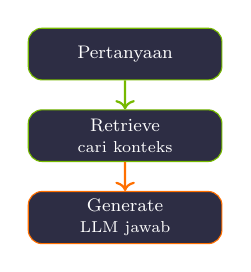
\begin{tikzpicture}[scale=0.82, every node/.style={transform shape},
          b/.style={draw=nvgreen, fill=nvcard, rounded corners=5pt, text=white, font=\footnotesize, minimum width=3cm, minimum height=0.8cm, align=center}]
        \node[b] (q) {Pertanyaan};
        \node[b, below=0.45cm of q] (r) {Retrieve\\\scriptsize cari konteks};
        \node[b, below=0.45cm of r, draw=nvorange] (g) {Generate\\\scriptsize LLM jawab};
        \draw[->,thick,color=nvgreen] (q)--(r);
        \draw[->,thick,color=nvorange] (r)--(g);
      \end{tikzpicture}
      \end{center}
    \end{column}
  \end{columns}
  \takeaway{RAG tak mengubah otak LLM --- ia \textbf{membekali} LLM konteks faktual segar sebelum menjawab.}
\end{frame}

% ── Analogi ───────────────────────────────────────────────
\begin{frame}{Analogi: Ujian Buka Buku}
  \framesubtitle{Menjawab sambil melihat sumber, bukan dari ingatan saja}
  \begin{columns}[T]
    \begin{column}{0.52\textwidth}
      \textcolor{nvred}{\textbf{Tutup buku}} (LLM polos):
      \begin{itemize}\footnotesize
        \item Jawab dari ingatan $\to$ mudah lupa / salah
      \end{itemize}
      \vspace{0.3em}
      \textcolor{nvgreen}{\textbf{Buka buku}} (RAG):
      \begin{itemize}\footnotesize
        \item Boleh buka halaman relevan dulu
        \item \textbf{Retrieve} $=$ menemukan halaman yang tepat
        \item Konteks dibekalkan ke LLM sebelum menjawab
        \item Jawaban bisa ditelusuri ke sumbernya
      \end{itemize}
    \end{column}
    \begin{column}{0.46\textwidth}
      \begin{center}
      \resizebox{0.9\linewidth}{!}{%
      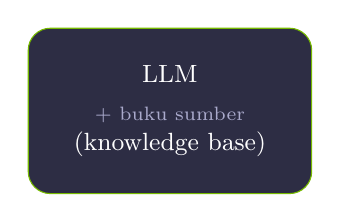
\begin{tikzpicture}
        \node[draw=nvgreen, fill=nvcard, rounded corners=8pt, text=white,
              font=\small, minimum width=3.6cm, minimum height=2.1cm, align=center]
              {LLM\\[0.3em]\scriptsize\color{nvgray}+ buku sumber\\(knowledge base)};
      \end{tikzpicture}}
      \end{center}
    \end{column}
  \end{columns}
  \takeaway{Dibekali konteks faktual dulu, baru menjawab --- bukan tebakan dari ingatan.}
\end{frame}

% ── Yang RAG ubah & tidak ──────────────────────────────────
\begin{frame}{Yang RAG Ubah --- dan Tidak}
  \framesubtitle{Harapan yang realistis}
  \begin{columns}[T]
    \begin{column}{0.49\textwidth}
      \textcolor{nvgreen}{\textbf{RAG membantu:}}
      \begin{itemize}\footnotesize
        \item[\textcolor{nvgreen}{\checkmark}] Jawaban berbasis dokumenmu
        \item[\textcolor{nvgreen}{\checkmark}] Update info $=$ update dokumen
        \item[\textcolor{nvgreen}{\checkmark}] Bisa beri \textbf{sitasi} sumber
        \item[\textcolor{nvgreen}{\checkmark}] Halusinasi \textbf{berkurang}
      \end{itemize}
    \end{column}
    \begin{column}{0.49\textwidth}
      \textcolor{nvred}{\textbf{RAG bukan sihir:}}
      \begin{itemize}\footnotesize
        \item[\textcolor{nvred}{$\bullet$}] Konteks salah $\to$ jawaban tetap meleset
        \item[\textcolor{nvred}{$\bullet$}] Halusinasi tak \textbf{hilang} 100\%
        \item[\textcolor{nvred}{$\bullet$}] Kualitas $=$ sebaik retrieval-nya
      \end{itemize}
    \end{column}
  \end{columns}
  \takeaway{``Garbage in, garbage out'': jawaban RAG hanya sebaik konteks yang berhasil ditemukan.}
\end{frame}

% ════════════════════════════════════════════════════════
\acttitle{2}{Anatomi RAG}{Embedding, pencarian makna, dan generator}

% ── Pipeline end-to-end ───────────────────────────────────
\begin{frame}{Alur End-to-End}
  \framesubtitle{Tiga langkah inti: embed $\to$ retrieve $\to$ generate}
  \begin{center}
    
\includegraphics[width=0.94\textwidth]{figures/rag_pipeline.png}
  \end{center}
  \takeaway{Pertanyaan di-\textbf{embed}, dicocokkan ke konteks, lalu LLM menjawab dari konteks itu.}
\end{frame}

% ── Embeddings ────────────────────────────────────────────
\begin{frame}{Embeddings: Makna Jadi Angka}
  \framesubtitle{Teks diubah jadi vektor; makna mirip $\to$ letak berdekatan}
  \begin{columns}[T]
    \begin{column}{0.5\textwidth}
      \begin{itemize}\footnotesize
        \item \textbf{Embedding}: teks $\to$ \textbf{vektor} (deretan angka)
        \item Kalimat \textbf{mirip makna} $\to$ vektor \textbf{berdekatan}
        \item Komputer membandingkan \textbf{jarak antar-angka}, bukan kata
        \item Model \textbf{multilingual} MiniLM $\to$ paham Bahasa Indonesia \emph{dan} Inggris
      \end{itemize}
    \end{column}
    \begin{column}{0.48\textwidth}
      \begin{center}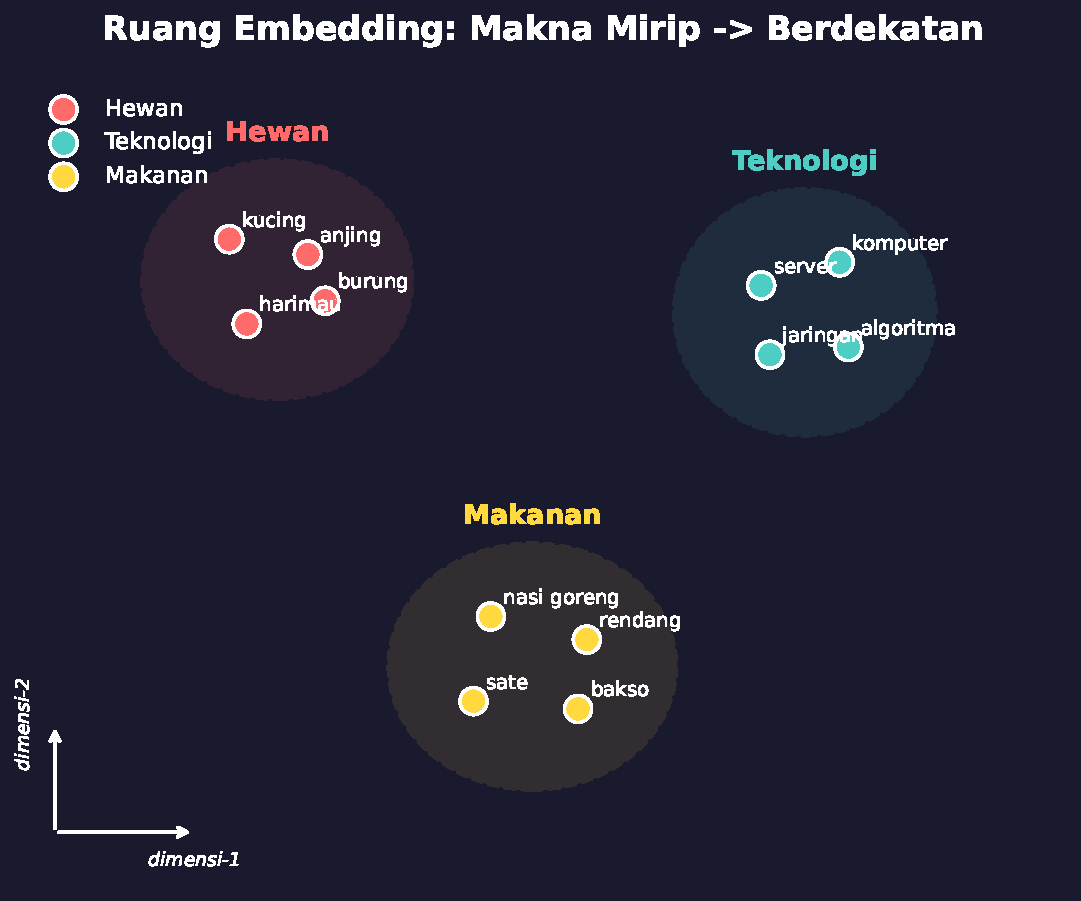
\includegraphics[width=0.72\linewidth]{figures/embedding_space.pdf}\end{center}
    \end{column}
  \end{columns}
  \takeaway{Embedding multilingual $=$ kunci pencarian \textbf{makna} lintas-bahasa (tanya ID, dokumen EN tetap ketemu).}
\end{frame}

% ── Semantic vs keyword ───────────────────────────────────
\begin{frame}{Pencarian Makna, Bukan Kata}
  \framesubtitle{Beda dengan Ctrl+F / pencarian kata kunci}
  \begin{columns}[T]
    \begin{column}{0.5\textwidth}
      \textcolor{nvred}{\textbf{Keyword (lexical)}}
      \begin{itemize}\footnotesize
        \item Cocokkan \textbf{kata persis}
        \item ``mobil'' $\ne$ ``kendaraan'' (beda kata)
        \item Sinonim \& parafrase lolos
      \end{itemize}
      \vspace{0.3em}
      \textcolor{nvgreen}{\textbf{Semantic (embedding)}}
      \begin{itemize}\footnotesize
        \item Cocokkan \textbf{makna}
        \item ``mobil'' $\approx$ ``kendaraan'' (vektor dekat)
      \end{itemize}
    \end{column}
    \begin{column}{0.48\textwidth}
      \begin{center}
      \begin{tikzpicture}[scale=0.9, every node/.style={transform shape}]
        \draw[->,color=nvgray] (-0.3,0)--(3.2,0);
        \draw[->,color=nvgray] (0,-0.3)--(0,2.6);
        \fill[nvgreen] (2.4,2.0) circle (3pt); \node[text=white,font=\scriptsize,right] at (2.5,2.0) {mobil};
        \fill[nvlightgreen] (2.1,1.7) circle (3pt); \node[text=white,font=\scriptsize,right] at (2.2,1.6) {kendaraan};
        \fill[nvorange] (0.5,0.4) circle (3pt); \node[text=white,font=\scriptsize,right] at (0.6,0.4) {pisang};
        \draw[<->,dashed,color=nvgray] (2.4,2.0)--(2.1,1.7);
      \end{tikzpicture}
      \end{center}
    \end{column}
  \end{columns}
  \takeaway{Semantic search menemukan dokumen relevan \textbf{walau pakai kata berbeda}.}
\end{frame}

% ── Augment & Generate ────────────────────────────────────
\begin{frame}{Augment \& Generate}
  \framesubtitle{Konteks disisipkan ke prompt, lalu LLM menjawab}
  \begin{columns}[T]
    \begin{column}{0.52\textwidth}
      \begin{itemize}\footnotesize
        \item \textbf{Augment}: gabung \textbf{konteks} hasil retrieve $+$ pertanyaan jadi satu prompt
        \item Format: bagian ``Konteks: \dots'' lalu ``Pertanyaan: \dots''
        \item \textbf{Generate}: LLM menyusun jawaban \textbf{hanya dari konteks}
        \item Instruksi kunci: ``bila tak ada di konteks, katakan tidak tahu'' $\to$ tekan karangan
      \end{itemize}
    \end{column}
    \begin{column}{0.46\textwidth}
      \begin{center}
      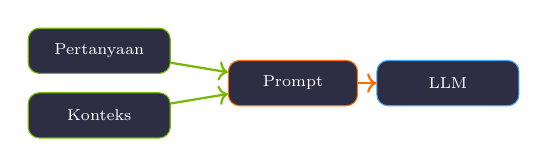
\begin{tikzpicture}[scale=0.82, every node/.style={transform shape},
          b/.style={draw=nvgreen, fill=nvcard, rounded corners=4pt, text=white, font=\scriptsize, minimum width=2.2cm, minimum height=0.7cm, align=center}]
        \node[b] (q) at (0,1) {Pertanyaan};
        \node[b] (c) at (0,0) {Konteks};
        \node[b, draw=nvorange, minimum width=2.0cm] (p) at (3,0.5) {Prompt};
        \node[b, draw=nvblue] (l) at (5.4,0.5) {LLM};
        \draw[->,thick,color=nvgreen] (q)--(p);
        \draw[->,thick,color=nvgreen] (c)--(p);
        \draw[->,thick,color=nvorange] (p)--(l);
      \end{tikzpicture}
      \end{center}
    \end{column}
  \end{columns}
  \takeaway{Augment $=$ jembatan retrieve $\to$ generate: konteks $+$ pertanyaan $\to$ satu prompt grounded.}
\end{frame}

% ════════════════════════════════════════════════════════
\acttitle{3}{Dari Dokumen ke Potongan}{Ingest dan chunking yang sadar-struktur}

% ── Ingest Docling ────────────────────────────────────────
\begin{frame}{Ingest: PDF $\to$ Teks Terstruktur}
  \framesubtitle{Docling membaca dokumen seperti manusia}
  \begin{columns}[T]
    \begin{column}{0.54\textwidth}
      \begin{itemize}\footnotesize
        \item PDF itu \textbf{visual} --- copy-paste teks sering berantakan
        \item \textbf{Docling} memparsing \textbf{struktur}: heading, paragraf, \textbf{tabel}
        \item \textbf{OCR} otomatis untuk halaman hasil scan / gambar
        \item Simpan \textbf{nomor halaman \& heading} tiap potongan
        \item Metadata itu $\to$ bahan baku \textbf{sitasi} nanti
      \end{itemize}
    \end{column}
    \begin{column}{0.44\textwidth}
      \begin{center}
      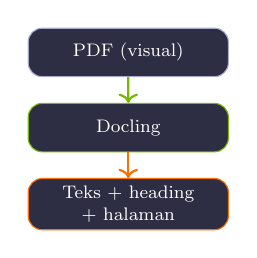
\begin{tikzpicture}[scale=0.82, every node/.style={transform shape},
          b/.style={draw=nvgreen, fill=nvcard, rounded corners=5pt, text=white, font=\footnotesize, minimum width=3.1cm, minimum height=0.75cm, align=center}]
        \node[b, draw=nvgray] (p) {PDF (visual)};
        \node[b, below=0.4cm of p] (d) {Docling};
        \node[b, below=0.4cm of d, draw=nvorange] (t) {Teks + heading\\+ halaman};
        \draw[->,thick,color=nvgreen] (p)--(d);
        \draw[->,thick,color=nvorange] (d)--(t);
      \end{tikzpicture}
      \end{center}
    \end{column}
  \end{columns}
  \takeaway{Ingest yang baik $=$ retrieval yang baik: struktur \& metadata terjaga sejak awal.}
\end{frame}

% ── Kenapa chunking ───────────────────────────────────────
\begin{frame}{Kenapa Dipotong (Chunking)?}
  \framesubtitle{Dokumen panjang dipecah jadi potongan kecil}
  \begin{itemize}\footnotesize
    \item Dokumen utuh \textbf{terlalu besar} untuk konteks LLM \& embedding (batas token)
    \item Retrieval per-\textbf{potongan} jauh lebih \textbf{presisi} daripada per-dokumen
    \item Tiap chunk $=$ satu unit makna yang bisa dicari \& disitasi
    \item Ukuran chunk disesuaikan \textbf{batas token embedder} (mis. 512)
  \end{itemize}
  \vspace{0.3em}
  \begin{center}
  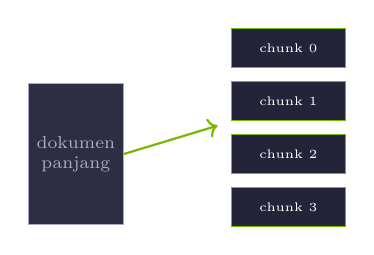
\begin{tikzpicture}[scale=0.9, every node/.style={transform shape}]
    \node[draw=nvgray, fill=nvcard, minimum width=1.0cm, minimum height=2.0cm, text=nvgray, font=\scriptsize, align=center] (doc) {dokumen\\panjang};
    \foreach \i/\y in {0/1.5,1/0.75,2/0,3/-0.75} {
      \node[draw=nvgreen, fill=nvdarkcard, minimum width=1.6cm, minimum height=0.55cm, font=\tiny, text=white] at (3,\y) {chunk \i};
    }
    \draw[->,thick,color=nvgreen] (doc.east) -- (2.0,0.4);
  \end{tikzpicture}
  \end{center}
  \takeaway{Chunk $=$ unit retrieval. Terlalu besar $\to$ kabur; terlalu kecil $\to$ konteks hilang.}
\end{frame}

% ── Strategi chunking ─────────────────────────────────────
\begin{frame}{Strategi Chunking}
  \framesubtitle{Beberapa cara memotong, dengan trade-off masing-masing}
  \begin{center}
  \renewcommand{\arraystretch}{1.3}{\footnotesize\setlength{\tabcolsep}{5pt}
  \begin{tabular}{@{}p{0.24\linewidth}p{0.40\linewidth}p{0.28\linewidth}@{}}
    \toprule \rowcolor{nvcard!50}
    \textbf{Strategi} & \textbf{Cara} & \textbf{Sifat} \\ \midrule
    Fixed (per-kata) & Potong tiap N kata + overlap & Sederhana, bisa putus kalimat \\
    Sentence & Pak kalimat utuh sampai batas & Rapi, ukuran bervariasi \\
    Semantic / struktur & Ikut paragraf \& heading (Docling \textbf{HybridChunker}) & Sadar-konteks, terbaik untuk sitasi \\
    \bottomrule
  \end{tabular}}
  \end{center}
  \takeaway{HybridChunker memotong \textbf{ikut struktur} dokumen --- dan menyimpan heading untuk sitasi.}
\end{frame}

% ════════════════════════════════════════════════════════
\acttitle{4}{Pencarian yang Lebih Baik}{Dua tahap: cepat dulu, akurat kemudian}

% ── Bi vs cross encoder ───────────────────────────────────
\begin{frame}{Bi-encoder vs Cross-encoder}
  \framesubtitle{Dua cara mengukur relevansi --- cepat vs akurat}
  \begin{columns}[T]
    \begin{column}{0.49\textwidth}
      \textcolor{nvgreen}{\textbf{Bi-encoder}}
      \begin{itemize}\footnotesize
        \item Embed query \& dokumen \textbf{terpisah}
        \item Bandingkan vektor (cepat, bisa di-index)
        \item Cocok untuk \textbf{ribuan} dokumen
        \item Kurang presisi pada nuansa
      \end{itemize}
    \end{column}
    \begin{column}{0.49\textwidth}
      \textcolor{nvorange}{\textbf{Cross-encoder}}
      \begin{itemize}\footnotesize
        \item Baca query \textbf{+} dokumen \textbf{bersama}
        \item Jauh lebih \textbf{akurat} menilai relevansi
        \item Lambat --- tak bisa di-index
        \item Hanya untuk \textbf{sedikit} kandidat
      \end{itemize}
    \end{column}
  \end{columns}
  \takeaway{Bi-encoder cepat menyaring banyak; cross-encoder teliti menilai sedikit. Gabungkan keduanya!}
\end{frame}

% ── Two-stage retrieval ───────────────────────────────────
\begin{frame}{Pencarian Dua Tahap}
  \framesubtitle{Over-fetch dengan bi-encoder, lalu rerank dengan cross-encoder}
  \begin{center}
    
\includegraphics[width=0.96\textwidth]{figures/two_stage_retrieval.png}
  \end{center}
  \takeaway{Ambil 20 kandidat cepat (bi-encoder) $\to$ urutkan ulang teliti (bge-reranker-v2-m3) $\to$ pakai 4 terbaik.}
\end{frame}

% ── Dampak rerank ─────────────────────────────────────────
\begin{frame}{Dampak Reranking}
  \framesubtitle{Tahap kedua mendongkrak presisi konteks}
  \begin{columns}[T]
    \begin{column}{0.42\textwidth}
      \begin{itemize}\footnotesize
        \item Reranker menilai \textbf{relevansi topik} dengan teliti
        \item Konteks lebih tepat $\to$ jawaban lebih \textbf{grounded}
        \item Biaya: sedikit lebih lambat per-query
        \item Jujur: reranker menilai \textbf{relevansi}, bukan jaminan jawaban ada di sana
      \end{itemize}
    \end{column}
    \begin{column}{0.56\textwidth}
      \begin{center}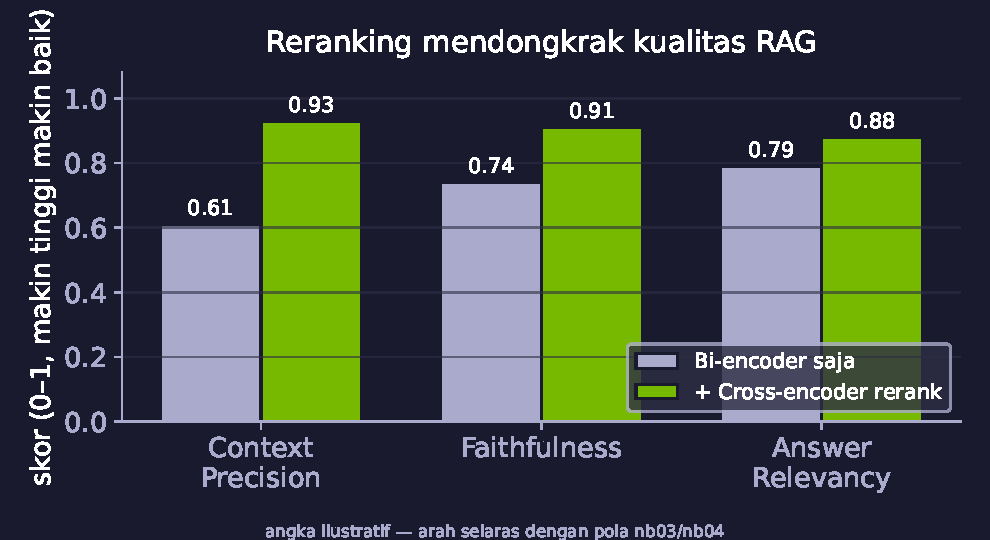
\includegraphics[width=\linewidth]{figures/rerank_lift.pdf}\end{center}
    \end{column}
  \end{columns}
\end{frame}

% ════════════════════════════════════════════════════════
\acttitle{5}{Apakah RAG-nya Bagus?}{Mengukur kualitas dengan RAGAS}

% ── 4 metrik RAGAS ────────────────────────────────────────
\begin{frame}{Empat Metrik RAGAS}
  \framesubtitle{Mengukur retrieval \emph{dan} jawaban --- bukan sekadar ``terasa benar''}
  \begin{center}
  \renewcommand{\arraystretch}{1.3}{\footnotesize\setlength{\tabcolsep}{5pt}
  \begin{tabular}{@{}p{0.30\linewidth}p{0.16\linewidth}p{0.46\linewidth}@{}}
    \toprule \rowcolor{nvcard!50}
    \textbf{Metrik} & \textbf{Menilai} & \textbf{Pertanyaannya} \\ \midrule
    Faithfulness & Jawaban & Apakah jawaban \textbf{setia} pada konteks (tak mengarang)? \\
    Answer Relevancy & Jawaban & Apakah jawaban \textbf{menjawab} pertanyaan? \\
    Context Precision & Retrieval & Apakah konteks yang diambil \textbf{relevan}? \\
    Context Recall & Retrieval & Apakah \textbf{semua} info yang dibutuhkan terambil? \\
    \bottomrule
  \end{tabular}}
  \end{center}
  \takeaway{Dua metrik menilai \textbf{retrieval}, dua menilai \textbf{jawaban} --- ukur keduanya untuk tahu di mana yang lemah.}
\end{frame}

% ── Judge LLM ─────────────────────────────────────────────
\begin{frame}{Siapa yang Menilai? LLM Judge}
  \framesubtitle{Model besar menilai jawaban model lain}
  \begin{columns}[T]
    \begin{column}{0.56\textwidth}
      \begin{itemize}\footnotesize
        \item RAGAS pakai \textbf{LLM judge} untuk menilai tiap metrik
        \item Judge harus \textbf{cukup pintar} --- model kecil sering gagal parsing JSON $\to$ skor NaN
        \item Kita pakai \textbf{NVIDIA NIM} (Llama-3.3-70B) sebagai judge $\to$ andal, tanpa GPU lokal
        \item Embedding metrik tetap lokal (multilingual MiniLM)
      \end{itemize}
    \end{column}
    \begin{column}{0.42\textwidth}
      \begin{center}
      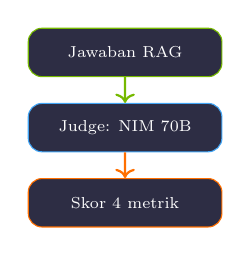
\begin{tikzpicture}[scale=0.82, every node/.style={transform shape},
          b/.style={draw=nvgreen, fill=nvcard, rounded corners=5pt, text=white, font=\scriptsize, minimum width=3.0cm, minimum height=0.75cm, align=center}]
        \node[b] (a) {Jawaban RAG};
        \node[b, below=0.4cm of a, draw=nvblue] (j) {Judge: NIM 70B};
        \node[b, below=0.4cm of j, draw=nvorange] (s) {Skor 4 metrik};
        \draw[->,thick,color=nvgreen] (a)--(j);
        \draw[->,thick,color=nvorange] (j)--(s);
      \end{tikzpicture}
      \end{center}
    \end{column}
  \end{columns}
  \takeaway{Judge yang lemah $=$ pengukuran yang menyesatkan. Pakai model judge yang kuat.}
\end{frame}

% ════════════════════════════════════════════════════════
\acttitle{6}{Menskalakan Index}{Recall vs kecepatan saat data membesar}

% ── Taksonomi index ───────────────────────────────────────
\begin{frame}{Taksonomi Index FAISS}
  \framesubtitle{Dari pencarian persis sampai perkiraan cepat}
  \begin{center}
  \renewcommand{\arraystretch}{1.3}{\footnotesize\setlength{\tabcolsep}{5pt}
  \begin{tabular}{@{}p{0.22\linewidth}p{0.44\linewidth}p{0.28\linewidth}@{}}
    \toprule \rowcolor{nvcard!50}
    \textbf{Index} & \textbf{Cara} & \textbf{Sifat} \\ \midrule
    Flat & Bandingkan ke \textbf{semua} vektor & Recall 100\%, lambat saat besar \\
    IVF & Bagi ruang jadi sel, cari sebagian (\texttt{nprobe}) & Cepat, recall sedikit turun \\
    HNSW & Graf tetangga berlapis & Sangat cepat, perkiraan \\
    \bottomrule
  \end{tabular}}
  \end{center}
  \takeaway{Cosine vs L2: untuk cosine, \textbf{normalisasi} dulu lalu pakai inner-product (IndexFlatIP).}
\end{frame}

% ── Trade-off recall vs speed ─────────────────────────────
\begin{frame}{Trade-off: Recall vs Kecepatan}
  \framesubtitle{Index perkiraan menukar sedikit akurasi untuk kecepatan}
  \begin{columns}[T]
    \begin{column}{0.4\textwidth}
      \begin{itemize}\footnotesize
        \item Data kecil $\to$ \textbf{Flat} sudah cukup (\& 100\% recall)
        \item Data besar $\to$ \textbf{IVF/HNSW} jauh lebih cepat
        \item Atur \texttt{nprobe} $\to$ geser recall vs kecepatan
        \item Simpan index ke disk (\texttt{write\_index}) --- muat saat start
      \end{itemize}
    \end{column}
    \begin{column}{0.58\textwidth}
      \begin{center}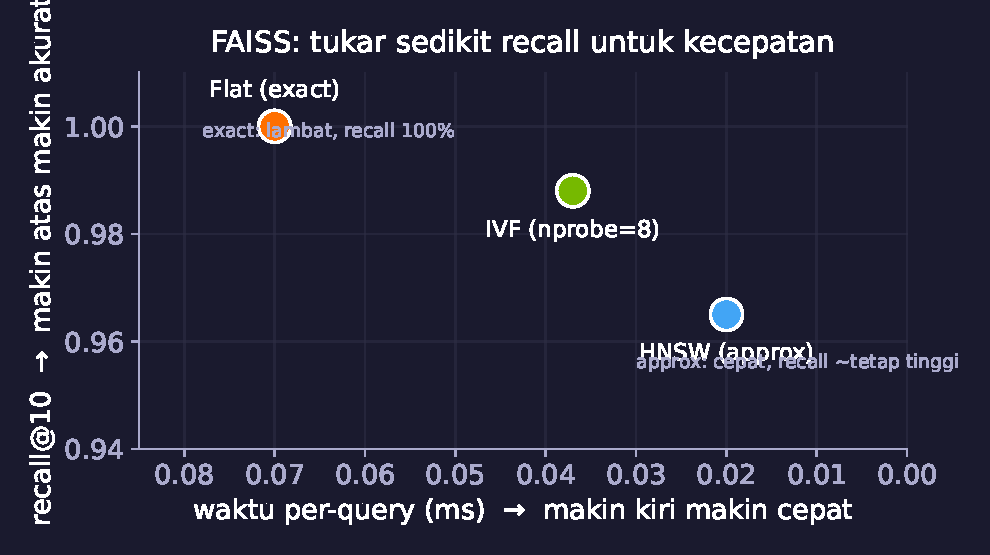
\includegraphics[width=\linewidth]{figures/faiss_tradeoff.pdf}\end{center}
    \end{column}
  \end{columns}
\end{frame}

% ── Persistence + Chroma ──────────────────────────────────
\begin{frame}{Persistence \& ChromaDB}
  \framesubtitle{Index yang awet, tak perlu dibangun ulang tiap start}
  \begin{itemize}\footnotesize
    \item \textbf{FAISS}: \texttt{write\_index} / \texttt{read\_index} $\to$ simpan \& muat dari disk
    \item \textbf{ChromaDB}: vector store dengan persistence otomatis (\texttt{PersistentClient})
    \item Bawa vektor sendiri (\texttt{embedding\_function=None}) $\to$ hindari unduh model ganda
    \item Pilih sesuai kebutuhan: FAISS (ringan, cepat) atau Chroma (metadata, filter)
  \end{itemize}
  \takeaway{Bangun index sekali, \textbf{simpan}, lalu muat saat start --- server tak rebuild tiap permintaan.}
\end{frame}

% ════════════════════════════════════════════════════════
\acttitle{7}{RAG yang Ingat}{Percakapan multi-giliran}

% ── Masalah pertanyaan lanjutan ───────────────────────────
\begin{frame}{Masalah Pertanyaan Lanjutan}
  \framesubtitle{Elipsis \& kata ganti membuat retrieval gagal}
  \begin{center}
  \renewcommand{\arraystretch}{1.3}{\footnotesize\setlength{\tabcolsep}{5pt}
  \begin{tabular}{@{}p{0.07\linewidth}p{0.42\linewidth}p{0.43\linewidth}@{}}
    \toprule \rowcolor{nvcard!50}
    \textbf{\#} & \textbf{Pertanyaan} & \textbf{Masalah} \\ \midrule
    1 & ``Berapa hari cuti tahunan?'' & Aman --- mandiri \\
    2 & ``Kalau cuti sakit?'' & \textbf{Elipsis} --- ``kalau'' merujuk giliran 1 \\
    3 & ``Perlu surat dokter?'' & \textbf{Kata ganti} implisit \\
    \bottomrule
  \end{tabular}}
  \end{center}
  \vspace{0.2em}
  \begin{center}\textcolor{nvred}{\small Embed ``Kalau cuti sakit?'' apa adanya $\to$ terlalu ambigu $\to$ retrieval meleset.}\end{center}
  \takeaway{Pertanyaan lanjutan harus dibuat \textbf{mandiri} dulu sebelum di-retrieve.}
\end{frame}

% ── Memori + rewriting ────────────────────────────────────
\begin{frame}{Memori + History-aware Rewriting}
  \framesubtitle{Tulis ulang jadi mandiri, lalu retrieve}
  \begin{center}
    
\includegraphics[width=0.96\textwidth]{figures/conversational_flow.png}
  \end{center}
  \takeaway{Memori \textbf{window} (giliran terbaru) $+$ \textbf{ringkasan} (giliran lama) $\to$ rewrite resolusi ``itu''/``-nya''.}
\end{frame}

% ════════════════════════════════════════════════════════
\acttitle{8}{Jawaban yang Bisa Dipercaya}{Sitasi dan verifikasinya}

% ── Sitasi ────────────────────────────────────────────────
\begin{frame}{Jawaban Bersitasi}
  \framesubtitle{Setiap klaim menunjuk sumbernya}
  \begin{columns}[T]
    \begin{column}{0.52\textwidth}
      \begin{itemize}\footnotesize
        \item Tiap konteks diberi label \texttt{[S1]..[S4]} $+$ halaman/heading
        \item LLM diminta \textbf{membubuhkan} label \texttt{[S\#]} pada klaim
        \item Pembaca bisa \textbf{menelusuri} klaim ke dokumen asli
        \item Ditampilkan: jawaban $+$ daftar \textbf{``Lihat sumber''}
      \end{itemize}
    \end{column}
    \begin{column}{0.46\textwidth}
      \begin{center}
      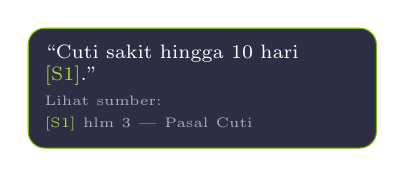
\begin{tikzpicture}[every node/.style={transform shape}]
        \node[draw=nvgreen, fill=nvcard, rounded corners=6pt, text=white, font=\scriptsize,
              text width=4.0cm, align=left, inner sep=6pt]
          {``Cuti sakit hingga 10 hari\\ \textcolor{nvlightgreen}{[S1]}.''\\[0.4em]
           \color{nvgray}\tiny Lihat sumber:\\ \textcolor{nvlightgreen}{[S1]} hlm 3 --- Pasal Cuti};
      \end{tikzpicture}
      \end{center}
    \end{column}
  \end{columns}
  \takeaway{Sitasi mengubah jawaban dari ``percaya saja'' menjadi ``\textbf{bisa diperiksa}''.}
\end{frame}

% ── Verifikasi sitasi ─────────────────────────────────────
\begin{frame}{Verifikasi Sitasi}
  \framesubtitle{Jangan percaya label yang ditulis model begitu saja}
  \begin{itemize}\footnotesize
    \item Model kecil bisa \textbf{mengarang} label (mis. \texttt{[S5]} padahal hanya ada 4)
    \item Kita \textbf{parse} label \texttt{[S\#]} dari jawaban, cek dalam rentang yang sah
    \item Label valid ditandai \textcolor{nvgreen}{\checkmark}; yang di luar daftar ditandai \textcolor{nvred}{$\triangle$} ``periksa!''
    \item Inilah inti capstone: jawaban yang \textbf{terverifikasi}, bukan sekadar terlihat rapi
  \end{itemize}
  \takeaway{``Trust, but verify'': tampilkan sumber \textbf{dan} cek labelnya secara otomatis.}
\end{frame}

% ════════════════════════════════════════════════════════
\acttitle{9}{Deploy}{Dari notebook ke layanan \texttt{/ask}}

% ── Deploy arch ───────────────────────────────────────────
\begin{frame}{RAG sebagai Layanan}
  \framesubtitle{Bungkus pipeline jadi API FastAPI \texttt{/ask}}
  \begin{center}
    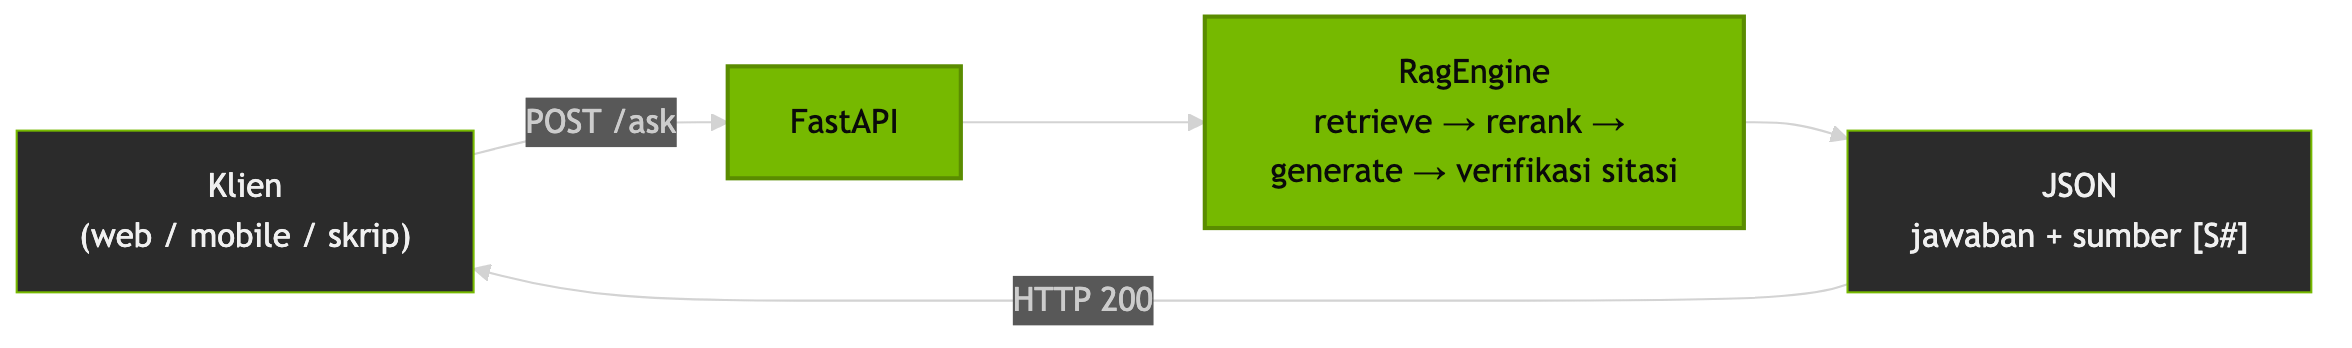
\includegraphics[width=0.96\textwidth]{figures/deploy_arch.png}
  \end{center}
  \takeaway{Model dimuat \textbf{sekali} saat start; tiap permintaan \texttt{/ask} balas \textbf{JSON} jawaban $+$ sumber (tervalidasi Pydantic).}
\end{frame}

% ── Generator cloud vs lokal ──────────────────────────────
\begin{frame}{Generator: Cloud vs Lokal}
  \framesubtitle{Satu sakelar, dua mode}
  \begin{center}
  \renewcommand{\arraystretch}{1.3}{\footnotesize\setlength{\tabcolsep}{5pt}
  \begin{tabular}{@{}p{0.22\linewidth}p{0.40\linewidth}p{0.30\linewidth}@{}}
    \toprule \rowcolor{nvcard!50}
    \textbf{Mode} & \textbf{Model} & \textbf{Kapan dipakai} \\ \midrule
    \textbf{NIM} (default) & NVIDIA NIM, Llama-3.3-70B (cloud) & Andal, \textbf{tanpa GPU} --- cocok untuk server \\
    \textbf{Qwen} (lokal) & Qwen2.5-3B 4-bit (T4) & Penuh on-prem / ber-GPU, tanpa API \\
    \bottomrule
  \end{tabular}}
  \end{center}
  \takeaway{Model besar (cloud) memberi rewriting \& jawaban lebih tajam --- \textbf{kualitas naik seiring kapasitas model}.}
\end{frame}

% ════════════════════════════════════════════════════════
\acttitle{10}{Ringkasan \& Peta}{Apa yang sudah dibangun, dan kapan memakai apa}

% ── Perjalanan 8 notebook ─────────────────────────────────
\begin{frame}{Perjalanan Modul 05}
  \framesubtitle{Delapan konsep, satu pipeline RAG yang lengkap}
  \begin{center}
  \renewcommand{\arraystretch}{1.18}{\scriptsize\setlength{\tabcolsep}{5pt}
  \begin{tabular}{@{}p{0.05\linewidth}p{0.40\linewidth}p{0.48\linewidth}@{}}
    \toprule \rowcolor{nvcard!50}
    \textbf{\#} & \textbf{Konsep} & \textbf{Inti} \\ \midrule
    1 & Fundamentals & embed $\to$ retrieve $\to$ generate \\
    2 & Ingest \& chunk & Docling + chunking sadar-struktur \\
    3 & Rerank & bi-encoder $\to$ cross-encoder \\
    4 & Ukur (RAGAS) & 4 metrik, judge NIM \\
    5 & Skala index & FAISS IVF/HNSW, ChromaDB \\
    6 & Conversational & memori + history-aware rewriting \\
    7 & Capstone & jawaban bersitasi terverifikasi \\
    8 & Deploy & layanan FastAPI \texttt{/ask} \\
    \bottomrule
  \end{tabular}}
  \end{center}
\end{frame}

% ── Panduan keputusan ─────────────────────────────────────
\begin{frame}{Panduan Keputusan}
  \framesubtitle{Kapan memakai apa}
  \begin{center}
  \renewcommand{\arraystretch}{1.3}{\footnotesize\setlength{\tabcolsep}{5pt}
  \begin{tabular}{@{}p{0.34\linewidth}p{0.60\linewidth}@{}}
    \toprule \rowcolor{nvcard!50}
    \textbf{Pertanyaan} & \textbf{Pegangan} \\ \midrule
    Ukuran chunk? & Sesuai batas token embedder (mis. 512), ikut struktur \\
    Perlu rerank? & Ya bila presisi konteks penting (hampir selalu) \\
    Index apa? & Kecil: Flat. Besar: IVF/HNSW + persistensi \\
    Generator apa? & Server tanpa GPU: NIM. On-prem GPU: lokal \\
    Percaya jawaban? & Hanya bila \textbf{ada sitasi} \& sitasi \textbf{terverifikasi} \\
    \bottomrule
  \end{tabular}}
  \end{center}
  \takeaway{RAG yang baik $=$ retrieval tepat $+$ jawaban grounded $+$ sumber yang bisa ditelusuri.}
\end{frame}

% ── Thank you ─────────────────────────────────────────────
\begin{frame}[plain]
  \vspace{2cm}
  \begin{center}
    {\color{nvgreen}\Huge\bfseries Terima Kasih!}\\[1.5em]
    {\color{nvgray}\Large Pertanyaan? Diskusi?}\\[2em]
    \begin{beamercolorbox}[rounded=true,shadow=false,sep=8pt,wd=10cm]{block body}
      \centering\color{white}
      \textbf{RAG Fundamentals} \quad $\cdot$ \quad Modul 05 \\
      Navasena Gen-ML Course
    \end{beamercolorbox}
  \end{center}
\end{frame}

\end{document}
